\section{Problem B - SDMA aspect}
\textit{Use the defined antenna patterns/directional signals from exercise A . You would need also some results/idea about exercise A2, if not finished (remember two main tasks : one to find C/I with directional spread signals, other to find shape of full radar sweep (effective antenna pattern wrt user and interferer) and resulting mean direction)}

\subsection{Question 1}
\textit{Now consider a 120 degree sector serviced with above antenna pattern in a SDMA operation (i.e. identical but offset patterns for N users). Consider the system to have power control so all users have same power received at the BS when the individual users antenna pattern maximum is pointed to their respective direction. Assume only a single path from user to BS (like exercise A1))}

\subsubsection{a and b) For a target C/I=9dB (spatial interference), what is the required user-to-interferer offset angle (to left and right)?. If C/I is 15 dB what then? and how many spatially separated users can be served in the sector, under the conditions mentioned in a)?. I.e. what is N=?}

The first approach made was trying to find the angle for which the radiation pattern presented a 12dB difference to its maximum. By doing this it was assured that when we added other users shifted to the left and to the right with the found angle, we would achieve a CIR of at least 9dB.

The first step was find the angle for which this 12dB difference was satisfied for the side lobe. In this way we are sure that we would have no more than 2 other users that are interfering (one to the left and one to he right). We found such angle was \SI{56}{\degree}. In \figref{fig:offset56deg} the setting is shown. It can be seen that 3 users can share the medium.

\begin{figure}[!h]
  \centering
  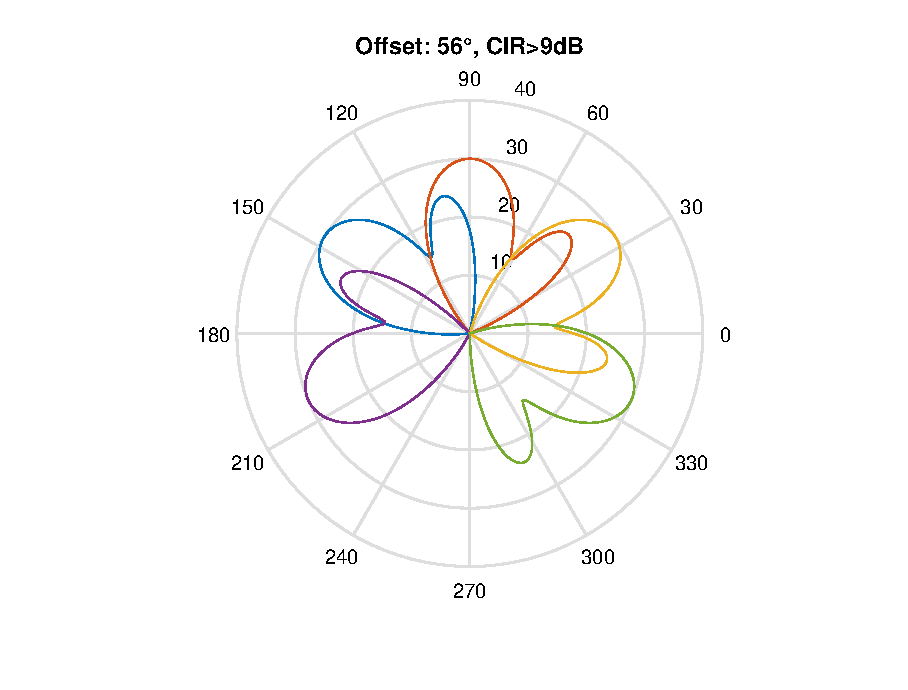
\includegraphics[width=11cm]{offset56deg.eps}
  \caption{Offset 56deg.}
  \label{fig:offset56deg}
\end{figure}

Then we realized that since the pattern was not symmetric, only one user was interfering, thus we could reduce the angle even more. We found it to be \SI{52.8}{\degree}. In \figref{fig:offset528deg} this new setting is shown. The medium can still be shared by 3 users.

\begin{figure}[!h]
  \centering
  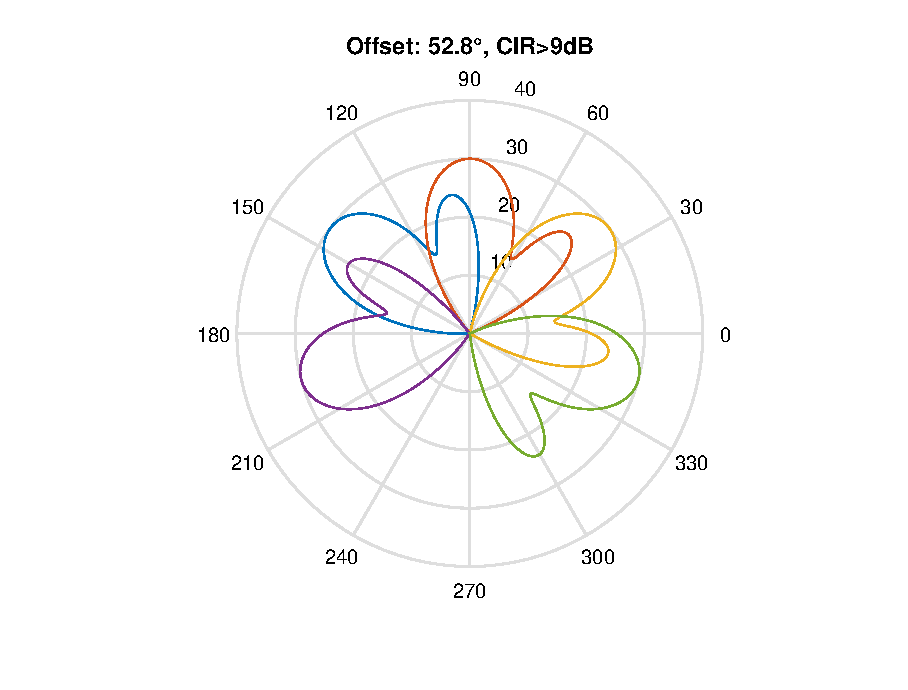
\includegraphics[width=11cm]{offset528deg.eps}
  \caption{Offset 52.8deg.}
  \label{fig:offset528deg}
\end{figure}

We thought also about finding the angle for which the 12dB difference was seen in the main lobe, this angle turned out to be \SI{24.5}{\degree}. As can be seen in \figref{fig:offset245deg} this leads to problems due to the non-symmetry of the pattern and the existence of the side lobe. The problems are present because instead of 2 interferers, we have 3.


\begin{figure}[!h]
  \centering
  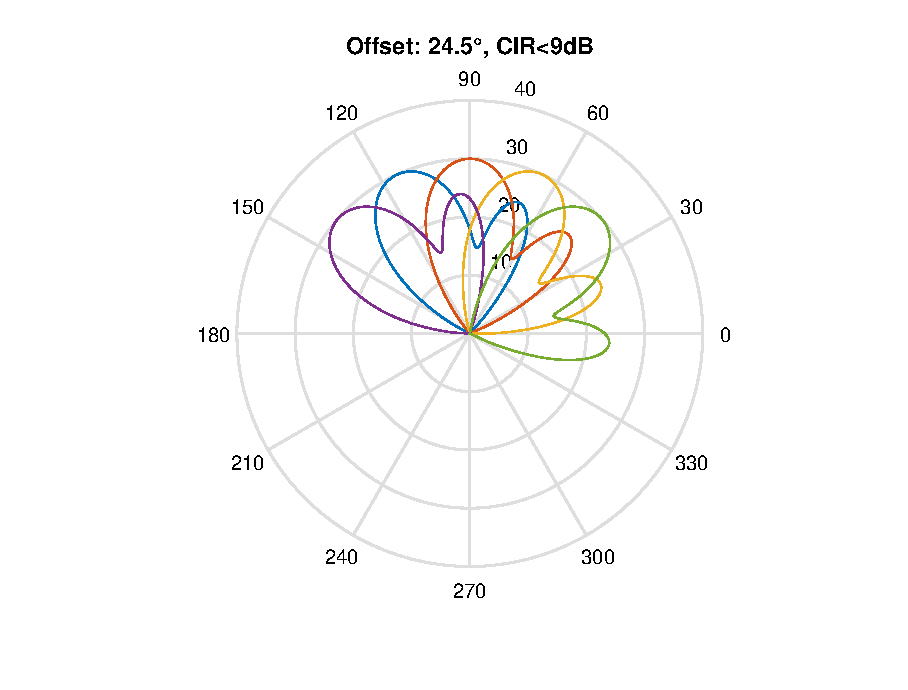
\includegraphics[width=11cm]{offset245deg.eps}
  \caption{Offset 24.5deg.}
  \label{fig:offset245deg}
\end{figure}

However if instead of considering the ``12dB point'' we take the angle in which the local minimum between the lobes is present (15dB point), then we could separate the users by \SI{29}{\degree} and achieve a big improvement: now 5 users can share the medium. This is shown in \figref{fig:offset29deg}.

\begin{figure}[!h]
  \centering
  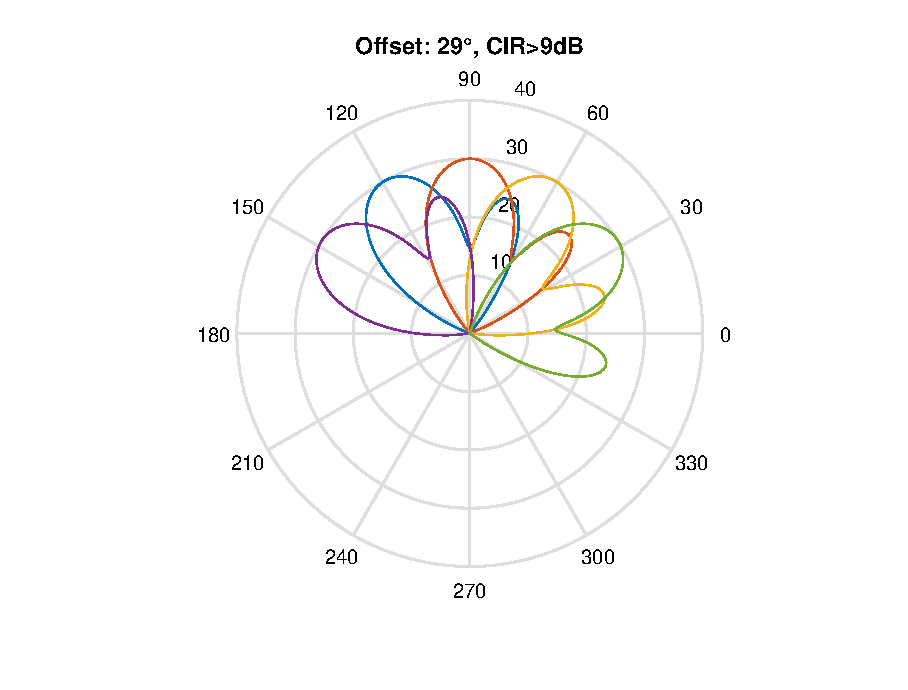
\includegraphics[width=11cm]{offset29deg.eps}
  \caption{Offset 29deg.}
  \label{fig:offset29deg}
\end{figure}


For the case of a required CIR of 15dB, a similar approach was made. We required to find an angle for which the difference between the main lobe was of 18dB. However, in this case we could not consider any angle in the main lobe, since none of them satisfied the condition, thus we had to find it in the outer part of the side lobe. We found this angle to be \SI{60}{\degree} as it is shown in \figref{fig:offset60deg}. This setting allows 3 users to share the medium.

\begin{figure}[!h]
  \centering
  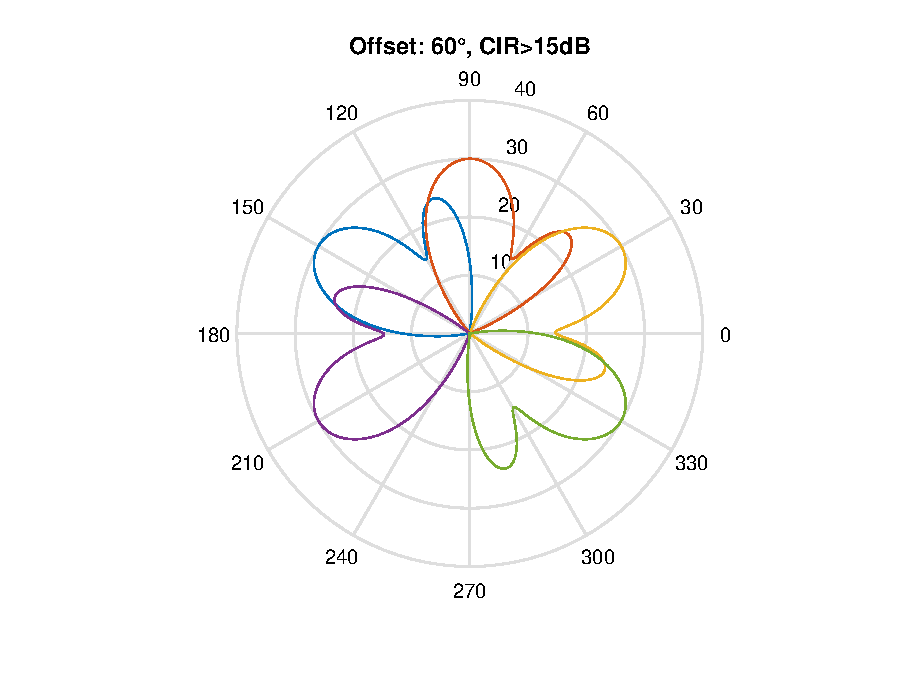
\includegraphics[width=11cm]{offset60deg.eps}
  \caption{Offset 60deg.}
  \label{fig:offset60deg}
\end{figure}

Similar to what was described above, we could decrease the require angle due to the asymmetric shape of the radiation pattern to a minimum angle of \SI{58}{\degree}. However as it is shown in \figref{fig:offset58deg}, this do not represent any improvement in the number of users that can share the medium; still only 3.

\begin{figure}[!h]
  \centering
  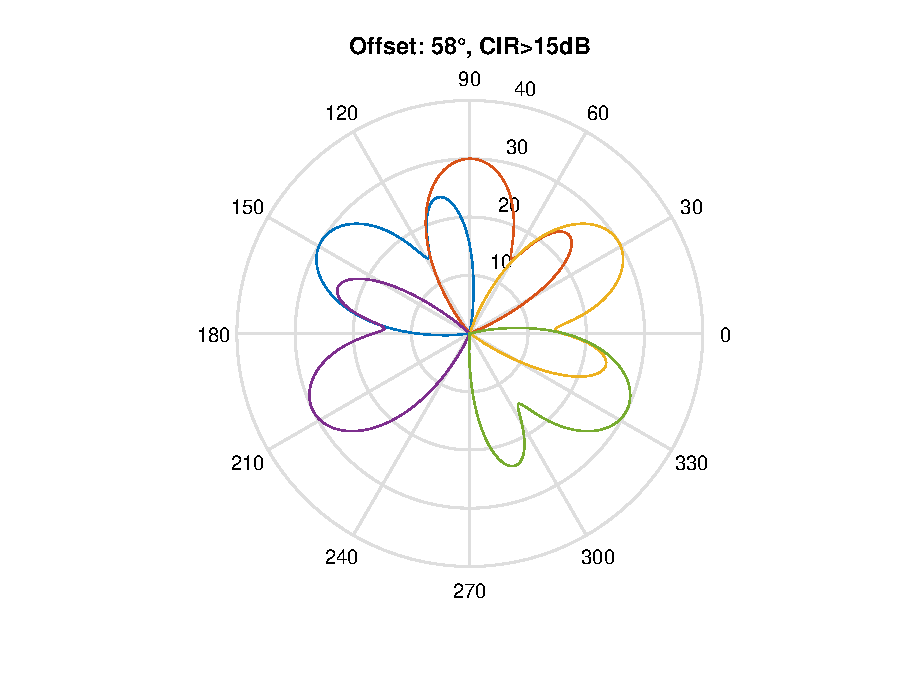
\includegraphics[width=11cm]{offset58deg.eps}
  \caption{Offset 58deg.}
  \label{fig:offset58deg}
\end{figure}

The \figref{fig:offset_angles} is shown as a reference to show all the mentioned angles in this section.

\begin{figure}[!h]
  \centering
  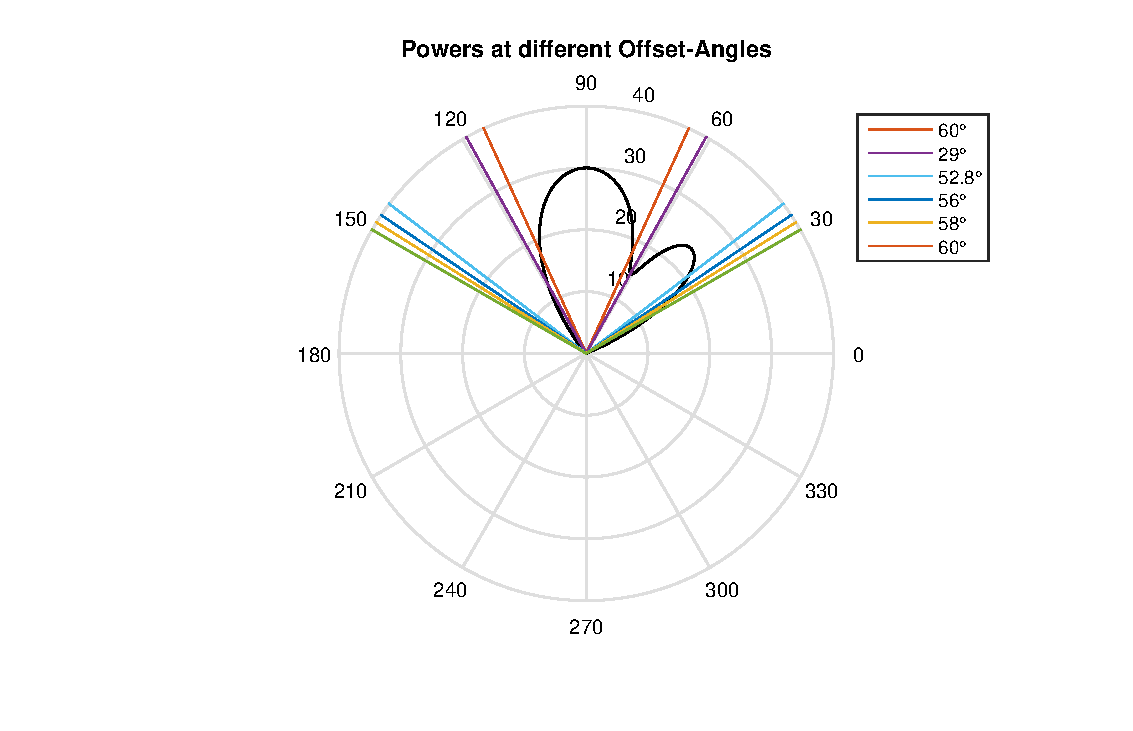
\includegraphics[width=12cm]{offset_angles.eps}
  \caption{Offset angles.}
  \label{fig:offset_angles}
\end{figure}

\subsection{Question 2}
\textit{Exchange the single path connections in exercise 1, to an angular uniform distribution over 20degree span and with a power density of 1 (similar to Cs in exercise A2). What changes result in the questions 1a) and 1b)?}

For this problem a similar approach than the made in the previous section was done, however, the pattern used for the calculations was the equivalent radiation pattern show in \figref{fig:equiv_rad_pat_mm4} which was the result of the convolution of the original pattern and the user distributed over \SI{20}{\degree}.

\begin{figure}[!h]
  \centering
  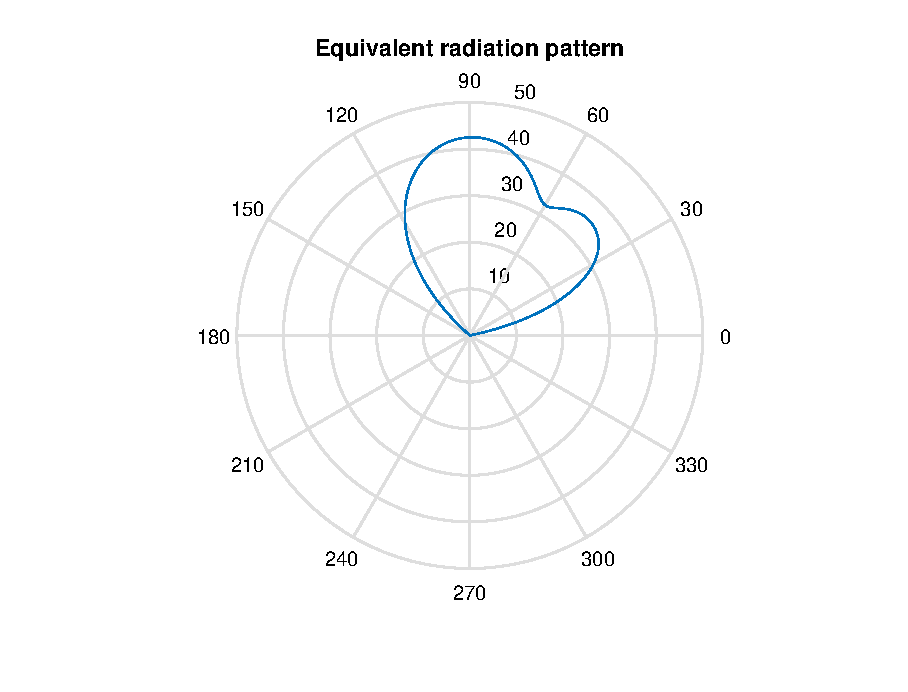
\includegraphics[width=12cm]{equiv_rad_pat_mm4.eps}
  \caption{Equivalent radiation pattern.}
  \label{fig:equiv_rad_pat_mm4}
\end{figure}

From what we learn from the case of single path scenario, we consider the angle for which the pattern shows a local minimum between the lobes, which is \SI{59}{\degree}. If we separate the users this angle, then as it is shown in \figref{fig:offset59deg} 3 users can share the medium.

\begin{figure}[!h]
  \centering
  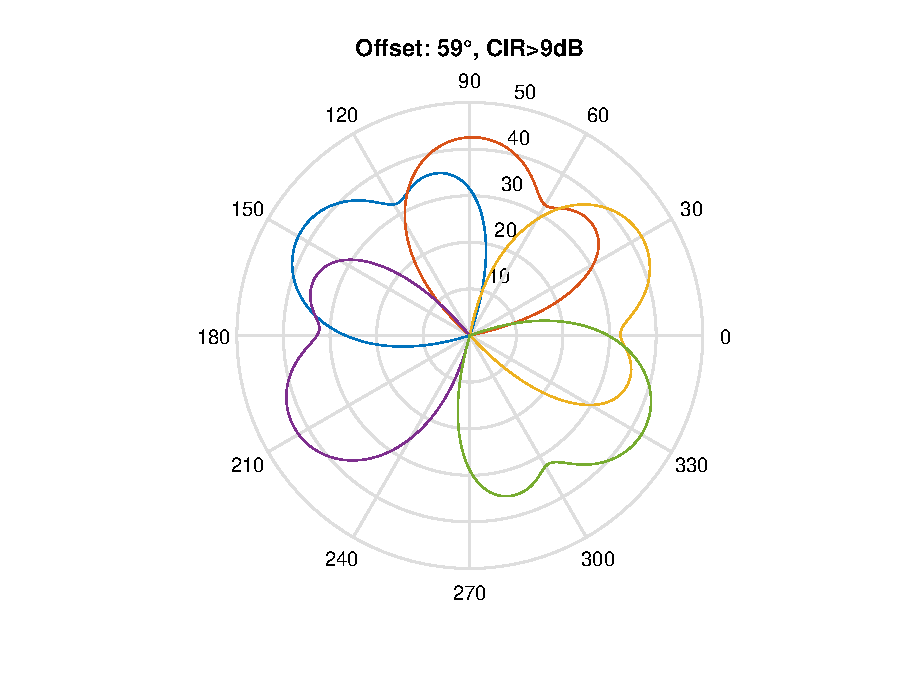
\includegraphics[width=12cm]{offset59deg.eps}
  \caption{Offset 59deg.}
  \label{fig:offset59deg}
\end{figure}

For a margin of -15dB, as shown in \figref{fig:offset633deg}, a separation angle of \SI{63.3}{\degree} is needed. This results in only 2 users being able to share the medium simultaneously.

\begin{figure}[!h]
  \centering
  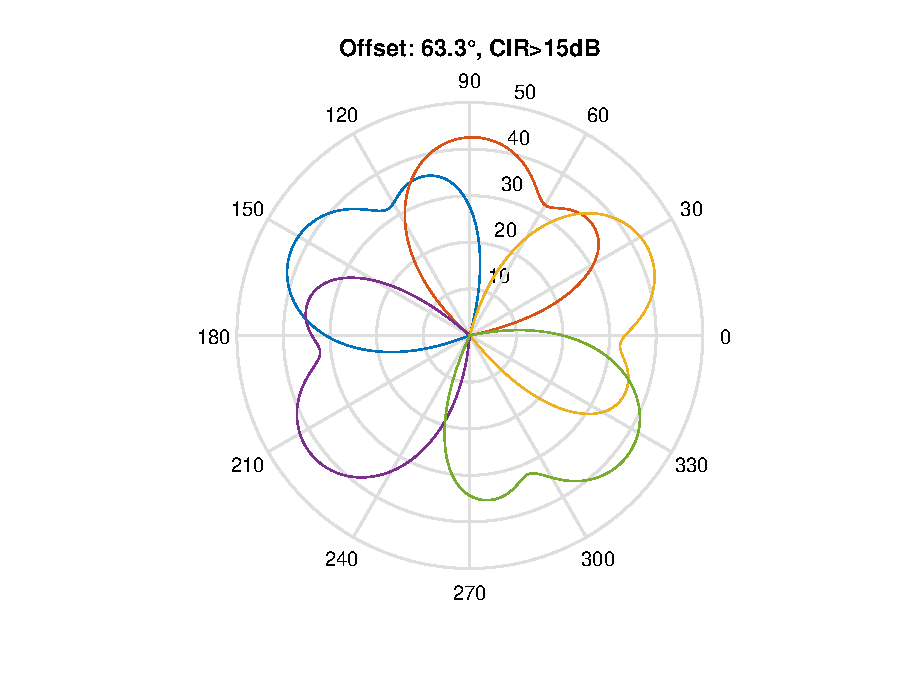
\includegraphics[width=12cm]{offset633deg.eps}
  \caption{Offset 63deg.}
  \label{fig:offset633deg}
\end{figure}